\section{Medical Imaging}
\label{section:medical-imaging}
At the beginning of \autoref{chapter:skelcl} we used the LM OSEM medical imaging application as our motivational example and application study to identify requirements for a high-level programming model.
In this section we will now study how we can express the LM OSEM application using algorithmic skeletons and how the parallel container data types and \SkelCL's redistribution feature simplify the programming of multi-\GPU systems.
We will start by briefly reintroducing the application and its sequential implementation before moving to the parallel implementation using first traditional \OpenCL and then \SkelCL for comparison.
A particular focus of this section will be on multi-\GPU systems and how \SkelCL drastically simplifies their programming.

\subsubsection*{The LM OSEM Algorithm}
\emph{List-Mode Ordered Subset Expectation Maximization} (LM OSEM)~\cite{ReaderErFlOt1998, SchellmannGoMeKoScWuBu2009} is a time-intensive, production-quality algorithm for medical image reconstruction.
LM OSEM takes a set of events from a PET scanner and splits them into $s$ equally sized subsets.
Then, for each subset $S_l, l \in {0, \ldots, s-1}$, the following computation is performed:
\begin{equation}
 f_{l+1}=f_{l}c_{l};\quad
 c_{l}=\dfrac{1}{A_N^T \textbf{1}}
\sum_{i \in S_{l}} (A_i)^T \dfrac{1}{A_{i} f_{l}}.
\label{eq:lm_osem2}
\end{equation}
Here $f$ is the 3D reconstruction image which is refined over time.
$A$ is a matrix where element $a_{ik}$ of row $A_i$ represents the length of intersection of the line between two PET detectors for a measured event $i$ with voxel $k$ of the reconstruction image.
The factor in front of the sum can be precomputed and is, therefore, omitted from here on.

\paragraph{Sequential implementation}
\autoref{lst:lmosem:seq_code:2} shows the sequential code for LM OSEM as already presented in \autoref{section:opencl-example}.
%
\begin{figure}
\begin{lstlisting}[
  caption={[Sequential code for LM OSEM.]Sequential code for LM OSEM comprises one outer loop with two nested inner loops.},
  label={lst:lmosem:seq_code:2}]
for (int l = 0; l < subsets; l++) {$\label{lst:lmosem:seq_core:2:loop}$
  // read subset

  // step 1: compute error image $c_l$
  for (int i = 0; i < subset_size; i++) { $\label{lst:lmosem:seq_code:2:step1:begin}$
    // compute $A_i$
    // compute local error
    // add local error to $c_l$
  } $\label{lst:lmosem:seq_code:step1:end}$

  // step 2: update reconstruction image $f$
  for (int k = 0 ; k < image_size; k++) { $\label{lst:lmosem:seq_code:2:step2:begin}$
    if (c_l[k] > 0.0) { f[k] = f[k] * c_l[k]; }
  } $\label{lst:lmosem:seq_code:2:step2:end}$
}
\end{lstlisting}
\end{figure}
%
The sequential LM OSEM is an iterative algorithm refining the reconstruction image $f$ over time.
At each iteration two major steps are performed:
\begin{itemize}
  \item[] \emph{Step 1:} the error image $c_l$ is computed by performing three sub-steps: 1) computation of the row $A_i$; 2) computing the local error for row $A_i$; 3) adding the local error to $c_l$;
  \item[] \emph{Step 2:} update the reconstruction image $f$ using the error image $c_l$ computed in Step 1.
\end{itemize}

\paragraph{Parallelization strategy}
For parallelization two possible decomposition strategies can be considered for the LM OSEM algorithm as initially suggested in~\cite{JonesJoKeNeReLeByBaMiCa2002}: Projection Space Decomposition (PSD) and Image Space Decomposition (ISD).

In PSD, the subsets $S_l$ are split into sub-subsets that are processed simultaneously while all processing units access a common reconstruction image $f$ and error image $c$.
Using this approach, we are able to parallelize \emph{Step~1} of the algorithm, but \emph{Step~2} is performed by a single processing unit.
On a multi-\GPU system, we have to copy the reconstruction image to all \GPUs before each iteration, and we have to merge all \GPUs' error images computed in \emph{Step~1} before proceeding with \emph{Step~2}.
While both steps are easy to implement, \emph{Step~2} does not efficiently use the available processing units.

In ISD, the reconstruction image $f$ is partitioned, such that each processing unit processes the whole subset $S_l$ with respect to a single part of the reconstruction image $f$.
Thus we are able to parallelize both steps of LM OSEM, but each processing unit still accesses the whole reconstruction image $f$ in order to compute the error value for each path before merging it with the error image $c$.
On a multi-\GPU system, the whole subset $S_l$ has to be copied to each \GPU in \emph{Step~1}.
ISD requires large amounts of memory (up to several GB in practically relevant cases) to save all paths computed in \emph{Step~1}.
Summarizing, it is hard to implement \emph{Step~1} on the \GPU, while \emph{Step~2} can be parallelized easily.

Therefore, we use a hybrid strategy for implementing LM OSEM:
\emph{Step~1} is parallelized using the PSD approach, while we use ISD for \emph{Step~2}.
This results in the sequence of five phases shown in \autoref{fig:lmosem:em_distribution2}:
\begin{enumerate}
\item \emph{Upload:} the subset ($S$) is divided into sub-subsets (one per \GPU).
      One sub-subset and the reconstruction image ($f$) are uploaded to each \GPU;
\item \emph{Step 1:} each \GPU computes the local error image ($c_l$) for its sub-subset;
\item \emph{Redistribution:} the local error images that are distributed on all \GPUs are downloaded and combined into a single error image on the host by performing element-wise addition.
      Afterwards, the combined error image and reconstruction image are partitioned, in order to switch the parallelization strategy from PSD to ISD.
      The corresponding parts of both images are distributed to the \GPUs again;
\item \emph{Step 2:} each \GPU updates its part of the reconstruction image;
\item \emph{Download:} finally, all parts of the reconstruction image are downloaded from the \GPUs to the host and merged into a single reconstruction image.
\end{enumerate}

\begin{figure}
  \centering
  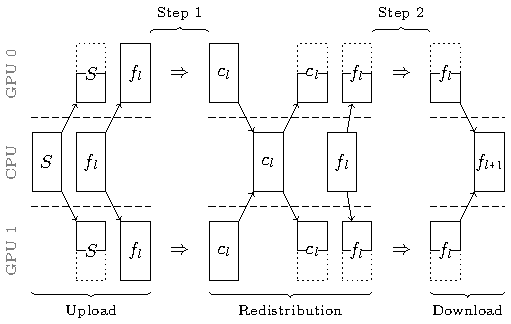
\includegraphics[width=0.6\textwidth]{ICCS/em_distribution}
  \caption{Parallelization schema of the LM OSEM algorithm.}
  \label{fig:lmosem:em_distribution2}
\end{figure}


\subsubsection*{\SkelCL Implementation}

The \SkelCL program in \autoref{lst:em_skelcl} reflects the described five phases in a concise, high-level manner, as shown by the corresponding comments.
The subset \code{s}, the error image \code{cl}, and the reconstruction image \code{f} are declared as \SkelCL vectors which enables an easy and automatic data transfer between \GPUs.
As data transfers are performed implicitly by \SkelCL, the upload phase is implemented by simply setting vector distributions (lines~\ref{lst:em:skelcl:upload:start}--\ref{lst:em:skelcl:upload:end}), while the download phase is performed implicitly when the \SkelCL containers are accessed or redistributed.
\begin{lstlisting}[%
  caption={SkelCL code of the LM OSEM algorithm},%
  numbers=left,%
float,%
label={lst:em_skelcl}]
auto computeCl = mapVector(
  [](Event e, const Vector<float>& f, Vector<float>& cl) {
    Path Ai = computeAi(e);$\label{lst:em:skelcl:computeAi}$
    float c = computeLocalError(f, Ai);
    addLocalErrorToCl(cl, c, Ai); });

auto updateF = zipVector(
  [](float f_i, float cl_i) {
    if (cl_i > 0.0) return f_i * cl_i; else return f_i; });

Vector<float> f   = readStartImage();
for (l = 0; l < subsets; l++) {
  Vector<Event> s = read_subset();
  Vector<float> cl(image_size);

  /* Upload */
  s.setDistribution(block);$\label{lst:em:skelcl:upload:start}$
  f.setDistribution(copy);
  cl.setDistribution(copy, add);$\label{lst:em:skelcl:upload:end}$

  /* Step 1: compute error image cl */
  computeCl(s, f, out(cl));$\label{lst:em:skelcl:execute}$

  /* Redistribution */
  f.setDistribution(block);$\label{lst:em:skelcl:redistribute:start}$
  cl.setDistribution(block);$\label{lst:em:skelcl:redistribute:end}$

  /* Step 2: update image estimate f */
  f = updateF(f, cl);

  /* Download (implicit) */}
\end{lstlisting}
The redistribution phase is implemented by changing the distributions of the corresponding \SkelCL containers (lines~\ref{lst:em:skelcl:redistribute:start} and~\ref{lst:em:skelcl:redistribute:end}).

The two computational steps are implemented using the \map and \zip skeleton from \SkelCL, correspondingly, as follows.

The first step -- the computation of the error image $c_l$ -- is implemented using the \map skeleton.
For each event \code{e} of the currently processed subset, the row $A_i$ is computed (line~\ref{lst:em:skelcl:computeAi}).
As $A_i$ is sparsely populated it is stored as a special data structure, called \code{Path}, to reduce its memory footprint.
Next, the local error is computed using $A_i$ together with the current reconstruction image $f$ which is passed to the \map skeleton as an additional argument.
Finally, the error image \code{cl} is updated with the local error.
The error image is also provided as an additional argument, but when executing the \map skeleton \code{cl} is wrapped using the \code{out} helper function (line~\ref{lst:em:skelcl:execute}).
This marks the additional argument as output parameter, \ie, the \SkelCL implementation is notified that this argument will be modified by the customizing function.
It is interesting to point out that the \map skeleton does not return a value, \ie, its return type is \code{void}.
The skeleton is only executed for its side effects on \code{cl}.

The second step -- the update of the reconstruction image $f$ -- is implemented using the \zip skeleton.
Here the customizing function operates on pairs of the voxels of the reconstruction and the error image, following the image space decomposition (ISD) strategy.
If the voxel of the error image is greater than zero, the voxel of the reconstruction image is updated with the product of the pair of voxels from the reconstruction and the error image.







\subsubsection*{Programming effort}
The lengthy and cumbersome \OpenCL implementation of the LM OSEM was already discussed in \autoref{chapter:skelcl}.
It is based on the work presented in~\cite{SchellmannGoMeKoScWuBu2009}.
\OpenCL requires a considerable amount of boilerplate code for running a kernel on multiple \GPUs, in particular for uploading and downloading data to and from the \GPUs.

The parallelization strategies are the same for both versions.
However, when using \SkelCL's vector data type, we avoid additional programming effort to implement data transfer between host and \GPU or between multiple \GPUs, and we obtain a multi-\GPU-ready implementation of LM OSEM for free.

\begin{figure}
  \centering
  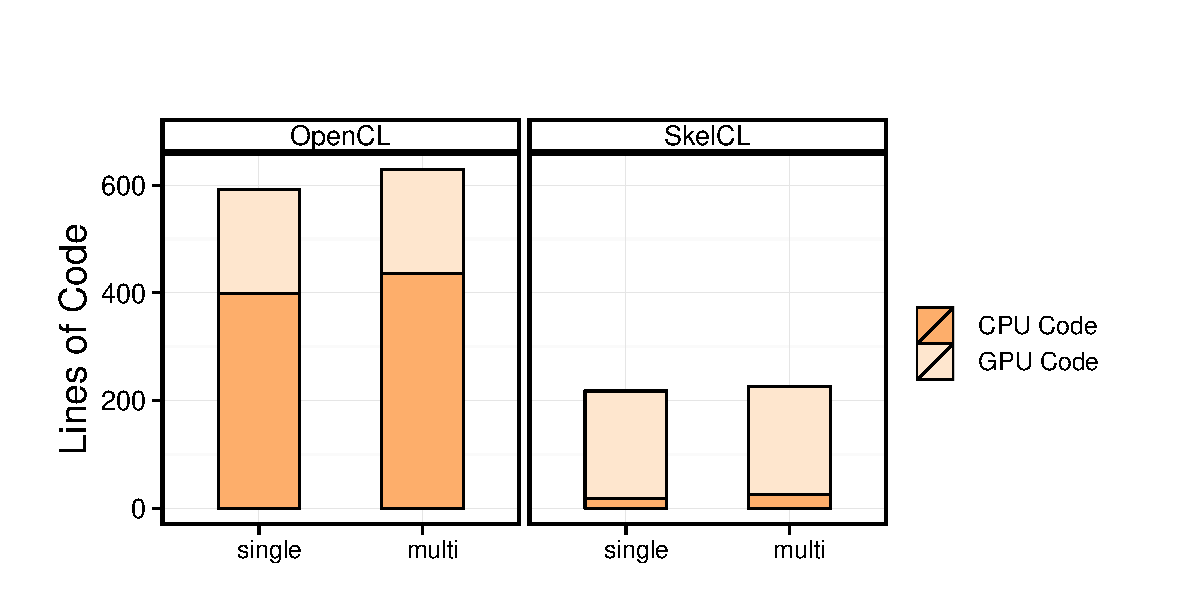
\includegraphics[width=.9\textwidth]{Plots/LMOSEM/lmosem_loc.pdf}
  \caption[Lines of code of the LM OSEM implementations.]%
          {Lines of code for \CPU and \GPU of the LM OSEM implementations on single- and multi-\GPU systems.}
  \label{fig:list-mode_OSEM:LOC}
\end{figure}

\autoref{fig:list-mode_OSEM:LOC} shows the lines of code required for both implementation.
The amount of lines required on the \GPU is similar.
This is not surprising, as these code describes the computation performed on the \GPU which is similar for both implementations.
The host code required for implementing the management of the \GPU execution differs significantly across implementations.
For a single \GPU, the \OpenCL-based implementation requires 206 LOCs, \ie, more than 11 times the number of lines than the \SkelCL program which has 18 LOCs.

Using multiple \GPUs in \OpenCL requires explicit code for additional data transfers between \GPUs.
This accounts for additional 37 LOCs for the \OpenCL-based implementation.
In \SkelCL, only 8 additional LOCs are necessary to describe the changes of data distribution.
These lines are easily recognizable in the \SkelCL program (lines~\ref{lst:em:skelcl:upload:start}--\ref{lst:em:skelcl:upload:end}, \ref{lst:em:skelcl:redistribute:start}--\ref{lst:em:skelcl:redistribute:end} in \autoref{lst:em_skelcl}, plus 3 lines during the initialization) and make this high-level code arguably better understandable and maintainable than the \OpenCL version.













\subsubsection*{Performance experiments}
We evaluated the runtimes of our two implementations of LM OSEM by reconstructing an image of $150\times 150\times 280$ voxels from a real-world PET data set with about $10^8$ events.
From this data set, about $10^2$ equally sized subsets are created.
In our experiments, we measured the average runtime of processing one subset.
To perform a full reconstruction producing a detailed reconstruction image, all subsets are processed multiple times, making LM OSEM a time-intensive application that runs several hours on a single-core \CPU.

\autoref{fig:list-mode_OSEM:runtime} shows the runtime of both implementations of LM OSEM using up to four \GPUs.
While the differences in the programming effort to implement the \SkelCL and \OpenCL versions are significant, the differences in runtime are quite small.
When running on a single \GPU, both implementations take the same time (3.66 seconds) to complete.
With two and four \GPUs, the \OpenCL implementation slightly outperforms the \SkelCL implementation, being 1.2\% and 4.7\% faster.
We presume that the slightly increasing overhead of \SkelCL is caused by the more complex data distribution performed when using more \GPUs.
Comparing to the significant reduction in programming effort, the runtime overhead of less than 5\% is arguably a moderate one.
In conclusion, this example shows that \SkelCL is suitable for implementing a real-world application and provides performance close to a native \OpenCL implementation.

\begin{figure}
  \centering
  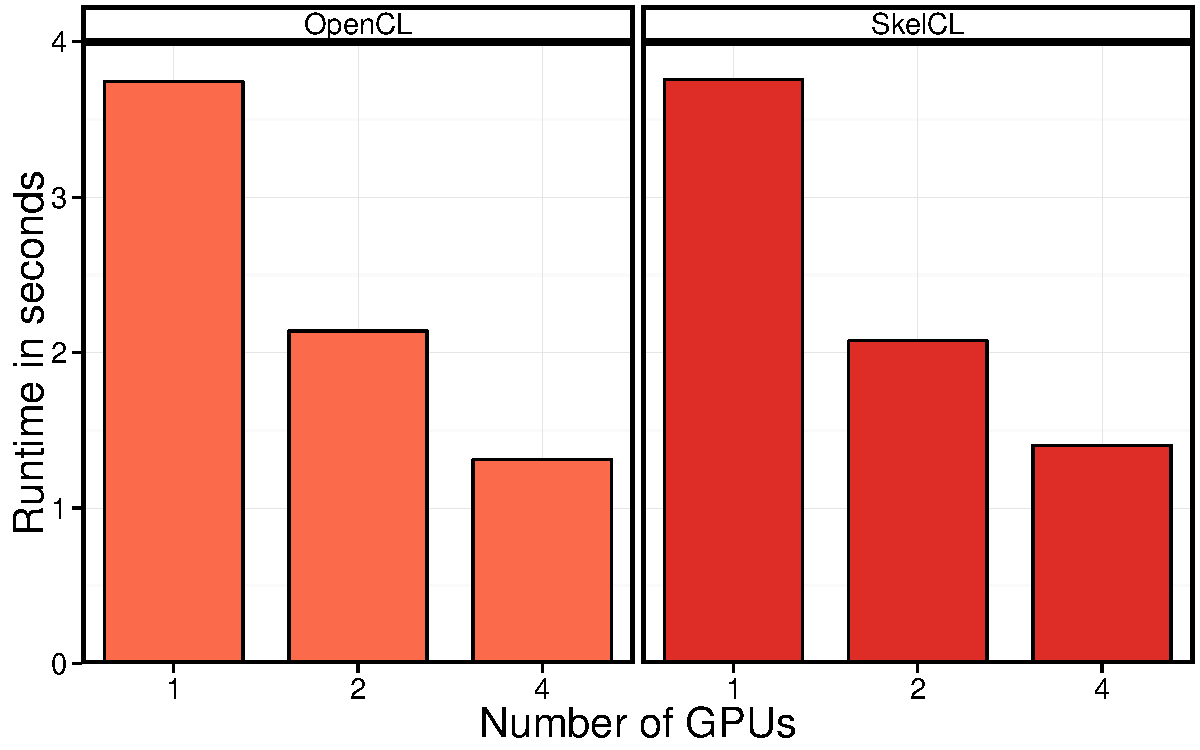
\includegraphics[width=.65\textwidth]{Plots/LMOSEM/lmosem_runtime.pdf}
  \caption[Average runtime of one iteration of the LM OSEM algorithm.]%
          {Average runtime of one iteration of the LM OSEM algorithm using \OpenCL and \SkelCL.}
  \label{fig:list-mode_OSEM:runtime}
\end{figure}

%\begin{figure}
%  \centering
%  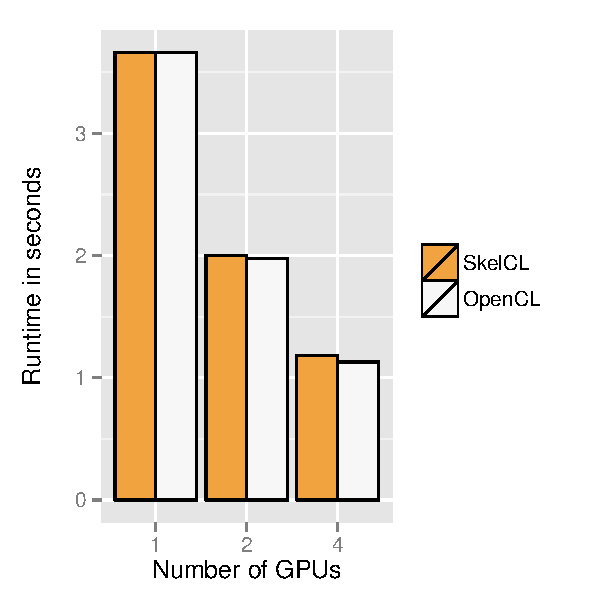
\includegraphics[width=.75\textwidth]{ICCS/skelcl-runtime.pdf}
%  \caption{Average runtime of one iteration of the LM OSEM algorithm using \SkelCL and \OpenCL.}
%  \label{fig:lmosem_runtime}
%\end{figure}

